\NeedsTeXFormat{LaTeX2e}
\documentclass[10pt,a4]{scrartcl}

\usepackage{tabularx,graphicx,a4,listings}

\ifx\pdfoutput\undefined
  % We're not running pdftex
  % european (better) fonts -- does not look good with pdflatex
  \usepackage[T1]{fontenc}
  \newcommand{\href}[2]{#2\\{\hspace*{5mm}\scriptsize <#1>}\\}
\else
  \pdfcompresslevel=9
  \def\pdfBorderAttrs{/Border [0 0 0] } % No border around Links
  \usepackage{hyperref}
\fi

\title{Equalizer Programming Guide}
\author{Stefan Eilemann\thanks{eile@eyescale.ch}\\[\medskipamount]
  % Eyescale Software Sarl
}
\date{
  \textbf{INCOMPLETE}\\[\medskipamount]
  Version 0.3, \today
}

\newcommand{\tm}{\texttrademark~}
\newcommand{\rc}{\raise 1ex\hbox{{\tiny\textregistered}}~}
\newcommand{\fig}[1]{Figure~\ref{#1}}

% suppress  single floating lines on top (widow) and bottom(club)
%  10000 is infinity
%  tradeoff: maybe underfull vboxes
\clubpenalty=10000
\widowpenalty=10000 

\begin{document}

\maketitle
\vfill
\lstset{language=C++}

\thispagestyle{empty}
\begin{figure}[ht]
  \hfill
  
\includegraphics[width=4cm]{logo.pdf}\hfill
  
\includegraphics[width=4cm]{vmml.pdf}\hfill\vspace{-1em}\\
%  {\small\htmladdnormallink{www.eyescale.ch}{http://www.eyescale.ch}}
\end{figure}
\vfill

%\abstract{
%  Equalizer is a project to develop software to simplify the creation of
%  scalable graphics applications and to improve the usability of
%  multipipe visualization systems.
%}

\vfill{\center\begin{tabularx}{\textwidth}{|l|l|X|}
    \hline
    \bf Version & \bf Date     & \bf Changes \\
    \hline
    0.3         & Aug 26, 2007 & application and render client code described\\
    0.2         & Aug 20, 2007 & main function described\\
    0.1         & Aug 19, 2007 & outlined the basic concepts\\
    \hline \multicolumn{3}{c}{\small
      \htmladdnormallink{http://www.equalizergraphics.com/documents/Developer/ProgrammingGuide.pdf}
      {http://www.equalizergraphics.com/documents/ProgrammingGuide.pdf}}\\
  \end{tabularx}}

\clearpage
\tableofcontents
\thispagestyle{empty}

\clearpage
\pagenumbering{arabic}

\section{Introduction}

Equalizer provides a framework for the development of parallel OpenGL
applications. Equalizer-based applications can run a single
shared-memory system with multiple graphics cards (GPU's) or on a
distributed graphics cluster. This Programming Guide introduces the
programming interface using the \textsf{eqPly} example shipped with Equalizer.

Any questions related to Equalizer programming and this Programming
Guide should be directed to the \textsf{eq-dev} mailing
list\footnote{see
  \htmladdnormallink{http://www.equalizergraphics.com/lists.html}
  {http://www.equalizergraphics.com/lists.html}}.

\section{Getting Started}

\subsection{Compiling and running \textsf{eqPly}}

A prerequisite for this Programming Guide is a working \textsf{eqPly}
example. The Quickstart
Guide\footnote{\htmladdnormallink{http://www.equalizergraphics.com/documents/EqualizerGuide.html}{http://www.equalizergraphics.com/documents/EqualizerGuide.html}}
explains how to run it. \textsf{eqPly} can also be executed without a
server, which simplifies the development cycle. In this case it will be
configured to use one window.

\subsection{Equalizer Processes}

\subsubsection{The Server}

An Equalizer server is responsible for managing one visualization
system\footnote{a shared memory system or graphics cluster}. Currently
it is only useful for running one application at a time, but it will be
extended to support multiple applications concurrently and efficiently
on one system. The server controls and potentially launches the
application's rendering clients.

\subsubsection{The Application}

The application connects to a server, which chooses a configuration for
the application. It provides a render client, to be launched by the
server. The application reacts on events and controls the rendering.

\subsubsection{The Render Client}

The render client implements the rendering part of an application. It is
passive, and receives all its rendering tasks from the server. The tasks
are executed by calling the appropriate task methods (see
\ref{ssTaskMethods}).

The application might be a rendering client, in which case it can also
contribute to the rendering. It can choose not to implement any render
client-related code, in which case it is reduced to be the application's
'master' process without any OpenGL windows.

The rendering client can be the same executable as the application, as
is the case with \textsf{eqPly}. Real-world applications often implement
a separate, light-weight rendering client.

\section{The Programming Interface}

Equalizer uses a C++ programming interface. The API is minimally
invasive, that is, Equalizer imposes only the minimal, natural execution
framework upon the application. It does not impose a scene graph or does
interfere in any way with the application's rendering code.

\subsection{\label{ssTaskMethods}Task Methods}

The application subclasses Equalizer objects and overrides virtual
functions to implement certain functionality, e.g., the application's
OpenGL rendering in \textsf{eq::Chan\-nel::frameDraw}. These task
methods are in concept similar to C function callbacks. The
\textsf{eqPly} section will discuss the most important task methods. A
full list of all task methods can be found on the
website\footnote{\htmladdnormallink{http://www.equalizergraphics.com/documents/design/taskMethods.html}{http://www.equalizergraphics.com/documents/design/taskMethods.html}}.

\subsection{The Resource Tree}

The rendering resources are represented in a hierarchical tree structure
which corresponds to the physical and logical resources found in a 3D
rendering environment. 

\begin{figure}[ht]
  \centering
  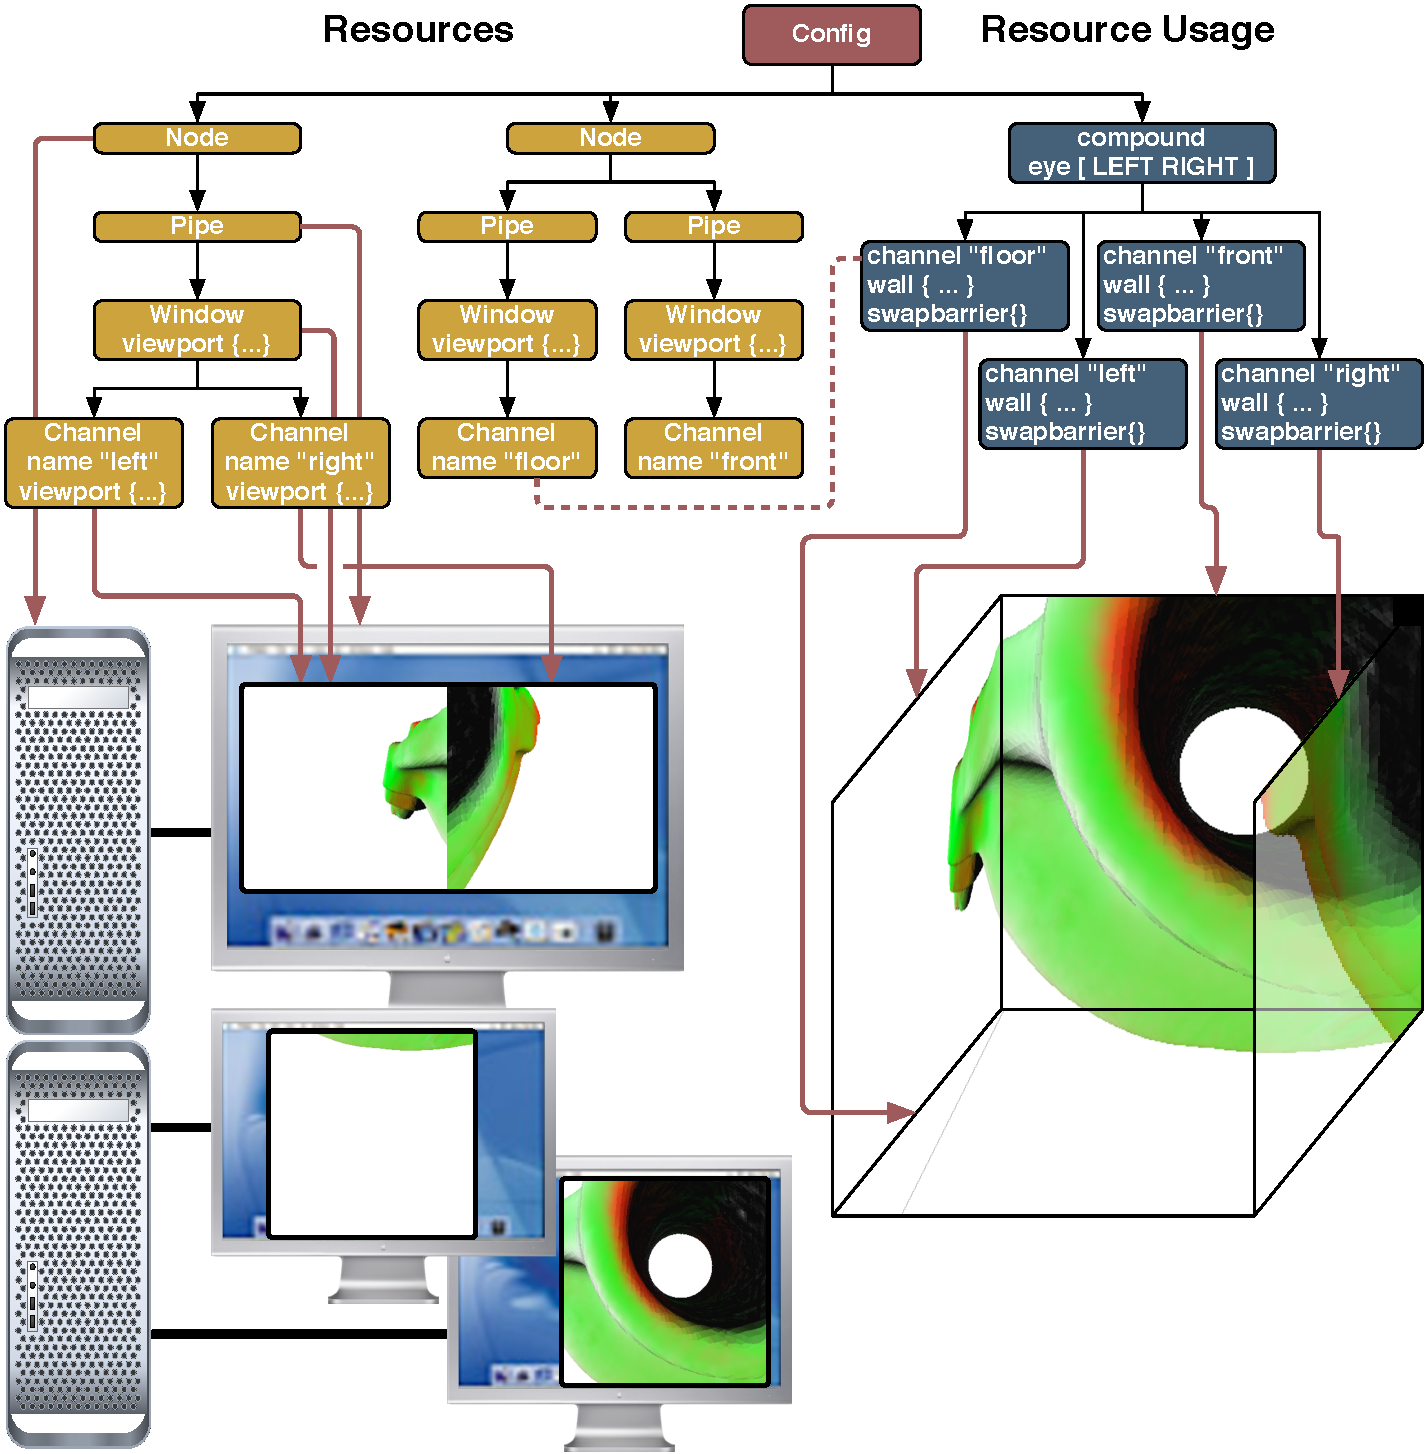
\includegraphics[width=\columnwidth]{cave.pdf}{\caption{\label{fConfig}An
      example configuration}}
\end{figure}

\fig{fConfig} shows one example configuration for a four-side
CAVE\texttrademark, running on two machines (node) using three graphics
cards (pipe) with one window each to render to the four output channels
connected to the projectors for each of the walls. The compound
description is only used by the server to compute the rendering
tasks. The application is not aware of compounds, and does not need to
concern itself with the parallel rendering logics of a configuration.

For testing and development purposes it is possible to use multiple
instances for one resource, e.g., to run multiple render client nodes on
one computer. For deployment one node and pipe should be used for each
computer and graphics card, respectively.

\subsubsection{Configuration}

The root of the resource tree is the \textsf{eq::Config}, which
represents the current configuration of the application. It currently
only holds the local node, not all nodes of the configuration.

\subsubsection{Node}

An \textsf{eq::Node} is the representation of a single computer in the
system. It is one operating system process of the render client. All
node task methods are executed from the main application thread.

\subsubsection{Pipe}

The \textsf{eq::Pipe} is the abstraction of a graphics card (GPU). In
the current implementation it is also one operating system thread,
unless the pipe's thread hint is set to \textsf{false}. All pipe and
child window and channel task methods are executed from the pipe thread
for threaded pipes or from the main application thread for non-threaded
pipes\footnote{see also
  \htmladdnormallink{http://www.equalizergraphics.com/documents/design/nonthreaded.html}{http://www.equalizergraphics.com/documents/design/nonthreaded.html}}.

Further versions of Equalizer might introduce threaded windows, where
all window-related task methods are executed in a separate operating
system thread.

\subsubsection{Window}

An \textsf{eq::Window} is an drawable and OpenGL context. The drawable
can be an on-screen window or an off-screen PBuffer or
FBO\footnote{off-screen drawables are not yet implemented, but can be
  created by the application and used with Equalizer}. 

\subsubsection{Channel}

The \textsf{eq::Channel} is the abstraction of an OpenGL viewport within
its parent window. It is the entity executing the actual rendering.

\subsection{Resource Usage}

How the rendering resources are to be used is configured using a
compound tree. Each compound has a channel, which it uses to execute the
rendering tasks. The rendering tasks are computed by the server and send
to the render clients. At no point the application or render clients
have or need knowledge of compounds. The configuration of compounds is
not in the scope of this document\footnote{see
  \htmladdnormallink{http://www.equalizergraphics.com/documents/design/compounds.html}{http://www.equalizergraphics.com/documents/design/compounds.html}}.

\section{The \textsf{eqPly} polygonal renderer}

The \textsf{eqPly} example is shipped with the Equalizer distribution
and serves as a simple reference implementation of an Equalizer-based
application. Its focus is not on rendering features or visual quality.
It serves as a test bed for most of the Equalizer features.

In this section the source code of \textsf{eqPly} is discussed in
detail, and relevant design decision and remarks are raised.

All classes in the example are in the \textsf{eqPly} namespace to avoid
type name ambiguities, in particular for the \textsf{Window} class.

\subsection{The main Function}

The main function starts off with parsing the command line into the
\textsf{LocalInitData} data structure, which in part will be distributed
to all render client nodes. For actual command line parsing is done by
the \textsf{LocalInitData} class and will be discussed there:

{\small\begin{lstlisting}
int main( int argc, char** argv )
{
    // 1. parse arguments
    eqPly::LocalInitData initData;
    initData.parseArguments( argc, argv );
\end{lstlisting}}

The second step is to initialize the Equalizer library. The
initialization function of Equalizer also parses the command line, which
is used to set certain default values based on Equalizer-specific
options\footnote{Equalizer-specific options always start with --eq-},
e.g., the default server location. Furthermore, a node factory is
provided. The \textsf{EQERROR} macro, and its counterparts
\textsf{EQWARN}, \textsf{EQINFO} and \textsf{EQVERB} allow selective
debugging outputs with various logging levels:

{\small\begin{lstlisting}
    // 2. Equalizer initialization
    NodeFactory nodeFactory;
    if( !eq::init( argc, argv, &nodeFactory ))
    {
        EQERROR << "Equalizer init failed" << endl;
        return EXIT_FAILURE;
    }
\end{lstlisting}}

The node factory is used by Equalizer to create the object instances for
the rendering entities. Each of the classes inherits from the same type
provided by Equalizer in the \textsf{eq} namespace. The provided
\textsf{eq::NodeFactory} base class instantiates a 'plain' Equalizer
object, thus making it possible to selectively subclass individual
entity types. For each rendering resource used in the configuration, one
C++ object will be created:

{\small\begin{lstlisting}
class NodeFactory : public eq::NodeFactory
{
public:
    virtual eq::Config*  createConfig()  { return new eqPly::Config; }
    virtual eq::Node*    createNode()    { return new eqPly::Node; }
    virtual eq::Pipe*    createPipe()    { return new eqPly::Pipe; }
    virtual eq::Window*  createWindow()  { return new eqPly::Window; }
    virtual eq::Channel* createChannel() { return new eqPly::Channel; }
};
\end{lstlisting}}

The third step is to create an instance of the application and to
initialize it locally. The application is an \textsf{eq::Client}, which
is an \textsf{eqNet::Node}. The underlying network distribution in
Equalizer is a peer-to-peer network structure of
\textsf{eqNet::Node}s. The application programmer rarely is aware of the
classes in the \textsf{eqNet} namespace, but both the
\textsf{eq::Client} and the server are \textsf{eqNet::Node}s. The local
initialization of nodes creates a local listening socket, so that the
node, and therefore the \textsf{eq::Client} can communicate over the
network with other nodes, such as the server and the rendering clients.

{\small\begin{lstlisting}
    // 3. initialization of local client node
    RefPtr< eqPly::Application > client = new eqPly::Application( initData );
    if( !client->initLocal( argc, argv ))
    {
        EQERROR << "Can't init client" << endl;
        eq::exit();
        return EXIT_FAILURE;
    }
\end{lstlisting}}

Finally everything is set up to run the \textsf{eqPly} application:

{\small\begin{lstlisting}
    // 4. run client
    const int ret = client->run();
\end{lstlisting}}

After it has finished, the application and Eqply is deinitialized and
the \textsf{main} function returns:

{\small\begin{lstlisting}
    // 5. cleanup and exit
    client->exitLocal();
    client = 0;

    eq::exit();
    return ret;
}
\end{lstlisting}}

\subsection{Application}

In the \textbf{eqPly} case, the application is also the render client. It has
three run-time behaviours:

\begin{enumerate}
  \item \textbf{Application}: The executable started by the user, which
    is the controlling entity in the rendering session.
  \item \textbf{Auto-launched render client}: The typical render client,
    started by the server. The server starts the executable with special
    parameters, which cause \textsf{Client::initLocal} to never
    return. During exit, the server terminates the process.
  \item \textbf{Resident render client}: Manually pre-started render
    client, listening on a specified port for server commands. This mode
    is selected using the command-line option \textsf{--eq-client} and
    potentially \textsf{--eq-listen} and \textsf{-r}\footnote{see \htmladdnormallink{http://www.equalizergraphics.com/documents/design/residentNodes.html}{http://www.equalizergraphics.com/documents/design/residentNodes.html}}.
\end{enumerate}

\subsubsection{Main Loop}

The application's main loop starts by connecting the application to an
Equalizer server. The command line parameter \textsf{--eq-server}
explicitly specifies a server address. If no server was specified,
\textsf{Client::connectServer} try first to connect to a server on the
local machine using the default port 4242. If that fails, it will create
a server running within the applications process with a default
1-channel configuration\footnote{see
  \htmladdnormallink{http://www.equalizergraphics.com/documents/design/standalone.html}{http://www.equalizergraphics.com/documents/design/standalone.html}}:

{\small\begin{lstlisting}
int Application::run()
{
    // 1. connect to server
    RefPtr<eq::Server> server = new eq::Server;
    if( !connectServer( server ))
    {
        EQERROR << "Can't open server" << endl;
        return EXIT_FAILURE;
    }
\end{lstlisting}}

The second step is to ask the server for a configuration. The
\textsf{ConfigParams} are a placeholder for later implementations to
provide additional hints and information to the server for choosing a
configuration. The configuration is created using
\textsf{NodeFactory::createConfig}. Therefore it is of type
\textsf{eqPly::Config}, but the return value is \textsf{eq::Config},
making q cast necessary:

{\small\begin{lstlisting}
    // 2. choose config
    eq::ConfigParams configParams;
    Config* config = static_cast<Config*>(server->chooseConfig( configParams ));

    if( !config )
    {
        EQERROR << "No matching config on server" << endl;
        disconnectServer( server );
        return EXIT_FAILURE;
    }
\end{lstlisting}}

Finally it is time to initialize the configuration. For statistics, the
time for this operation is measures and printed. During initialization
the server launches and connects all render client nodes, and calls the
appropriate initialization task methods, as explained in later
sections. \textsf{Config::init} does return after all nodes, pipes,
windows and channels are initialized. It returns \textsf{true} only if
all init task methods were successful. The \textsf{EQLOG} macro allows
topic-specific logging. The numeric topic values are specified in the
respective \textsf{log.h} header files:

{\small\begin{lstlisting}
    // 3. init config
    eqBase::Clock clock;

    config->setInitData( _initData );
    if( !config->init( ))
    {
        EQERROR << "Config initialization failed: " 
                << config->getErrorMessage() << endl;
        server->releaseConfig( config );
        disconnectServer( server );
        return EXIT_FAILURE;
    }

    EQLOG( eq::LOG_CUSTOM ) << "Config init took " << clock.getTimef() << " ms"
                            << endl;
\end{lstlisting}}

When the configuration was successfully initialized, the actual main
loop is executed. The main loop runs until the user exits the
configuration or a maximum number of frames, specified as a command-line
argument, has been rendered. The latter is useful for benchmarks. The
\textsf{Clock} is reused for measuring the overall performance. A new
frame is started using \textsf{Config::startFrame} and a frame is
finished using \textsf{Config::endFrame}.

When the frame is started, the server computes all rendering tasks and
sends them to the appropriate render client nodes. The render client
nodes dispatch the tasks to the correct node or pipe thread, were they
are executed in the order they arrive.

The frame finished is \textsf{latency} frames behind the frame
started. The latency is specified in the configuration file, and allows
several outstanding frames whose tasks are already queued in the node
and pipe threads for execution. This allows overlapped execution and
minimizes idle times.

When the main loop is finished, \textsf{Config::finishAllFrames} catches
up with the latency. It returns after all outstanding frames have been
rendered:

{\small\begin{lstlisting}
    // 4. run main loop
    uint32_t maxFrames = _initData.getMaxFrames();
    
    clock.reset();
    while( config->isRunning( ) && maxFrames-- )
    {
        config->startFrame();
        // config->renderData(...);
        config->finishFrame();
    }
    const uint32_t frame = config->finishAllFrames();
    const float    time  = clock.getTimef();
    EQLOG( eq::LOG_CUSTOM ) << "Rendering took " << time << " ms (" << frame
                            << " frames @ " << ( frame / time * 1000.f)
                            << " FPS)" << endl;
\end{lstlisting}}

The remainder of the application code cleans up in the reverse order of
the initialization. The config is exited, released and the connection to
the server is closed:

{\small\begin{lstlisting}
    // 5. exit config
    clock.reset();
    config->exit();
    EQLOG( eq::LOG_CUSTOM ) << "Exit took " << clock.getTimef() << " ms" <<endl;

    // 6. cleanup and exit
    server->releaseConfig( config );
    if( !disconnectServer( server ))
        EQERROR << "Client::disconnectServer failed" << endl;
    server = 0;
    return EXIT_SUCCESS;
}
\end{lstlisting}}

\subsubsection{Render Clients}

In the second and third case, when the executable is used as a render
client, \textsf{Client::initLocal} never returns. In order to keep the
client resident, the \textsf{eqPly} example overrides the client loop to
keep it running beyond one configuration run:

{\small\begin{lstlisting}
bool Application::clientLoop()
{
    if( !_initData.isResident( )) // execute only one config run
        return eq::Client::clientLoop();

    // else execute client loops 'forever'
    while( true ) // TODO: implement SIGHUP handler to exit?
    {
        if( !eq::Client::clientLoop( ))
            return false;
        EQINFO << "One configuration run successfully executed" << endl;
    }
    return true;
}
\end{lstlisting}}


\if 0
{\small\begin{lstlisting}
\end{lstlisting}}
\fi

\end{document}
